\section{AutoPas Software}

AutoPas is a C++ library specifically designed to optimize short-range particle simulations through dynamic algorithm selection. It acts as a black box, where users provide the specifications while the library handles the choice of the best suitable algorithm through auto-tuning. By periodically evaluating various algorithms, AutoPas ensures that the most efficient configuration is applied as simulation conditions change. The library includes example applications, such as the md-flexible framework, which will be used in the course of this thesis \parencite{gratl2019autopas}.


\subsection{Data layouts}

AutoPas supports two primary data layouts for storing particle information in memory: Array of Structures (AoS) and Structure of Arrays (SoA). In the AoS layout, each particle is represented as an object containing all its properties, such as position and force, stored together in memory. This arrangement allows for efficient cache utilization when accessing individual particles, but can limit vectorization efficiency. On the other hand, the SoA layout separates particle properties into individual arrays, with each array containing data for all particles, leading to better vectorization by aligning data contiguously in memory. However, this layout may lead to less efficient cache usage when accessing properties of a single particle \parencite{gratl2019autopas}.

\subsection{Neighbor identification algorithms} \label{sec:neighbor_iden_algs}

During auto-tuning AutoPas has to decide how to manage and store the particles of the simulation, and most importantly how to identify the neighboring particles to efficiently compute the pairwise forces. As shown in section \ref{sec:shortrange}, for each particle, the particles within the cut-off radius should be found, and the rest will be ignored. This process is repeated for every single particle in the container, and choosing the right Neighbor identification algorithm, is crucial when it comes to performance. Below, the four algorithms used in AutoPas are presented. These algorithms are implemented as containers in AutoPas, managing neighbor identification and the overall particle organization, including the selection of the data layout. 

\subsubsection{Direct Sum}

The straightforward, and thus naive, approach, is to calculate the distances from one particle to all other particles without utilizing any additional data structures. Instead, all particles are stored in a single cell, and for each particle, distances to all other particles are evaluated to determine whether they fall within the cutoff radius. Forces are only computed for pairs of particles within this radius. As illustrated in \hyperref[fig:directsum]{Figure \ref*{fig:directsum}}, the red particle represents the current particle, for which forces are being calculated, the red circle denotes the cutoff radius, and the arrows depict the interactions between the current particle and the others.

This method, while eliminating the complexity and overhead associated with bigger data structures, is computationally inefficient. The calculation of pairwise forces results in a time complexity of \(O(n^2)\), where \(n\) is the number of particles \parencite{gratl2022n}. Although simple, this approach is only practical for simulations with a very small number of particles.


\subsubsection{Linked Cells}

This approach extends the Direct Sum method by dividing the simulation domain into cells, with each cell containing the particles within its boundaries. The cell dimensions are set to at least the cutoff radius (\(r_c\)). This ensures that short-range interactions are computed only between particles in the current cell and its eight neighboring cells, as depicted with blue in \hyperref[fig:linkedcells]{Figure \ref*{fig:linkedcells}}.

Because the cell size matches the cutoff radius, particles outside these neighboring cells are guaranteed to lie beyond the interaction range and can be excluded from force calculations. For homogeneous particle distributions, this reduces the computational complexity from \(O(n^2)\) to \(O(n)\) \parencite{knapek2007numerical}. Furthermore, Linked Cells improve cache efficiency by storing particles within the same cell contiguously in memory. 

Nonetheless, there is still computational overhead, as around 84.5\% of the particles in the search region are outside the cutoff radius, leading to redundant distance calculations. The probability of finding a pair of particles within the cutoff radius in a 3D simulation, is approximately 15.5\% and can be estimated using the following equation \parencite{gratl2019autopas}:

\[
\frac{\textit{Cutoff volume}}{\textit{Search volume}_{LC}} =
\frac{\frac{4}{3} \pi r_c^3}{(3r_c)^3}
\]

\subsubsection{Verlet Lists} \label{sec:verletlists}

The idea behind Verlet Lists is to precompute and store neighbor lists for each particle. This allows the AutoPas to efficiently track all nearby particles within a particle's cutoff radius, making pairwise interaction calculations faster by reducing the number of distance checks needed in each iteration.

Since particles move during the simulation, these lists eventually become outdated and need to be rebuilt whenever a new particle enters or leaves the cutoff region. To reduce how often these lists need to be rebuilt, an additional safety margin is introduced, known as the Verlet skin factor \(s\). The cutoff radius \(r_c\) is scaled by this factor, expanding the search radius to \(r_c \cdot s\), as shown with yellow in Figure~\ref{fig:verletlists}. This extended region allows the neighbor lists to remain valid for multiple iterations, reducing the frequency of rebuilds.

With this approach, the probability of finding a particle in the cutoff region in a 3D simulation domain is given by \parencite{gratl2019autopas}:

\[
\frac{\textit{Cutoff volume}}{\textit{Search volume}_{VL}} =
\frac{\frac{4}{3} \pi r_c^3}{\frac{4}{3} \pi (r_c \cdot s)^3} =
\frac{1}{s^3}.
\]


Selecting an appropriate skin factor is crucial, as it affects both the number of unnecessary calculations and how often the neighbor lists are rebuilt. For instance, a skin factor of 1.2 reduces the number of unnecessary distance calculations by half compared to Linked Cells.

Throughout the simulation, as particles move, two cases arise:
\begin{itemize}
    \item If a particle moves away from another, it may remain in the neighbor list longer than necessary, increasing storage costs and unnecessary force calculations.
    \item If a particle moves closer to another, it may enter its cutoff radius but not be included in the neighbor list, leading to incorrect force calculations.
\end{itemize}

To avoid these issues, AutoPas uses a fixed rebuild frequency parameter, ensuring that all neighbor lists are rebuilt every \(N\) iterations to keep them compact and accurate. 


On top of that, when using dynamic containers as described in \parencite{gall2023exploration}, the maximum particle displacement per iteration is used as a metric of when to rebuild. In this case the displacement of each particle from its last rebuild position is tracked in every iteration. This displacement is then compared to a threshold, which is chosen as half of the Verlet skin size \parencite{thompson2022lammps}. If at least one particle exceeds this threshold, it could have entered the cutoff region of another particle, and therefore the neighbor lists are rebuilt.


To improve efficiency, AutoPas builds the Verlet Lists algorithm on top of Linked Cells. Therefore, the neighbor lists are constructed by assessing only particles in neighboring cells. This allows the computational complexity to be reduced from \(O(N^2)\) (brute-force search) to \(O(N)\) \parencite{yao2004improved}. 

Verlet Lists are particularly effective for systems with high particle densities. However, their lack of spatial locality can lead to inefficient memory access, resulting in poor cache performance and reduced vectorization efficiency \parencite{gratl2022n}.


\subsubsection{Verlet Cluster Lists}

Verlet Cluster Lists are built upon regular Verlet Lists by grouping particles into clusters rather than maintaining individual neighbor lists for each particle Figure~\ref{fig:verletclusters}. This approach reduces memory overhead, as a single neighbor list is created for each cluster instead of one for every particle. The algorithm uses the observation that neighboring particles often share similar neighbor lists, allowing $M$ particles to be combined into a cluster. When two clusters are close, all interactions between the particles within these clusters are calculated. This optimization decreases the number of neighbor lists by a factor of $\frac{1}{M}$ \parencite{gratl2022n}, and enhances computational efficiency by enabling better vectorization. However, the increased search radius, can lead to additional distance calculations. Despite this, Verlet Cluster Lists are well-suited for large systems with high particle densities.

\begin{figure}[h!]
    \centering
    % First Figure
    \begin{subfigure}{0.22\textwidth}
        \centering
        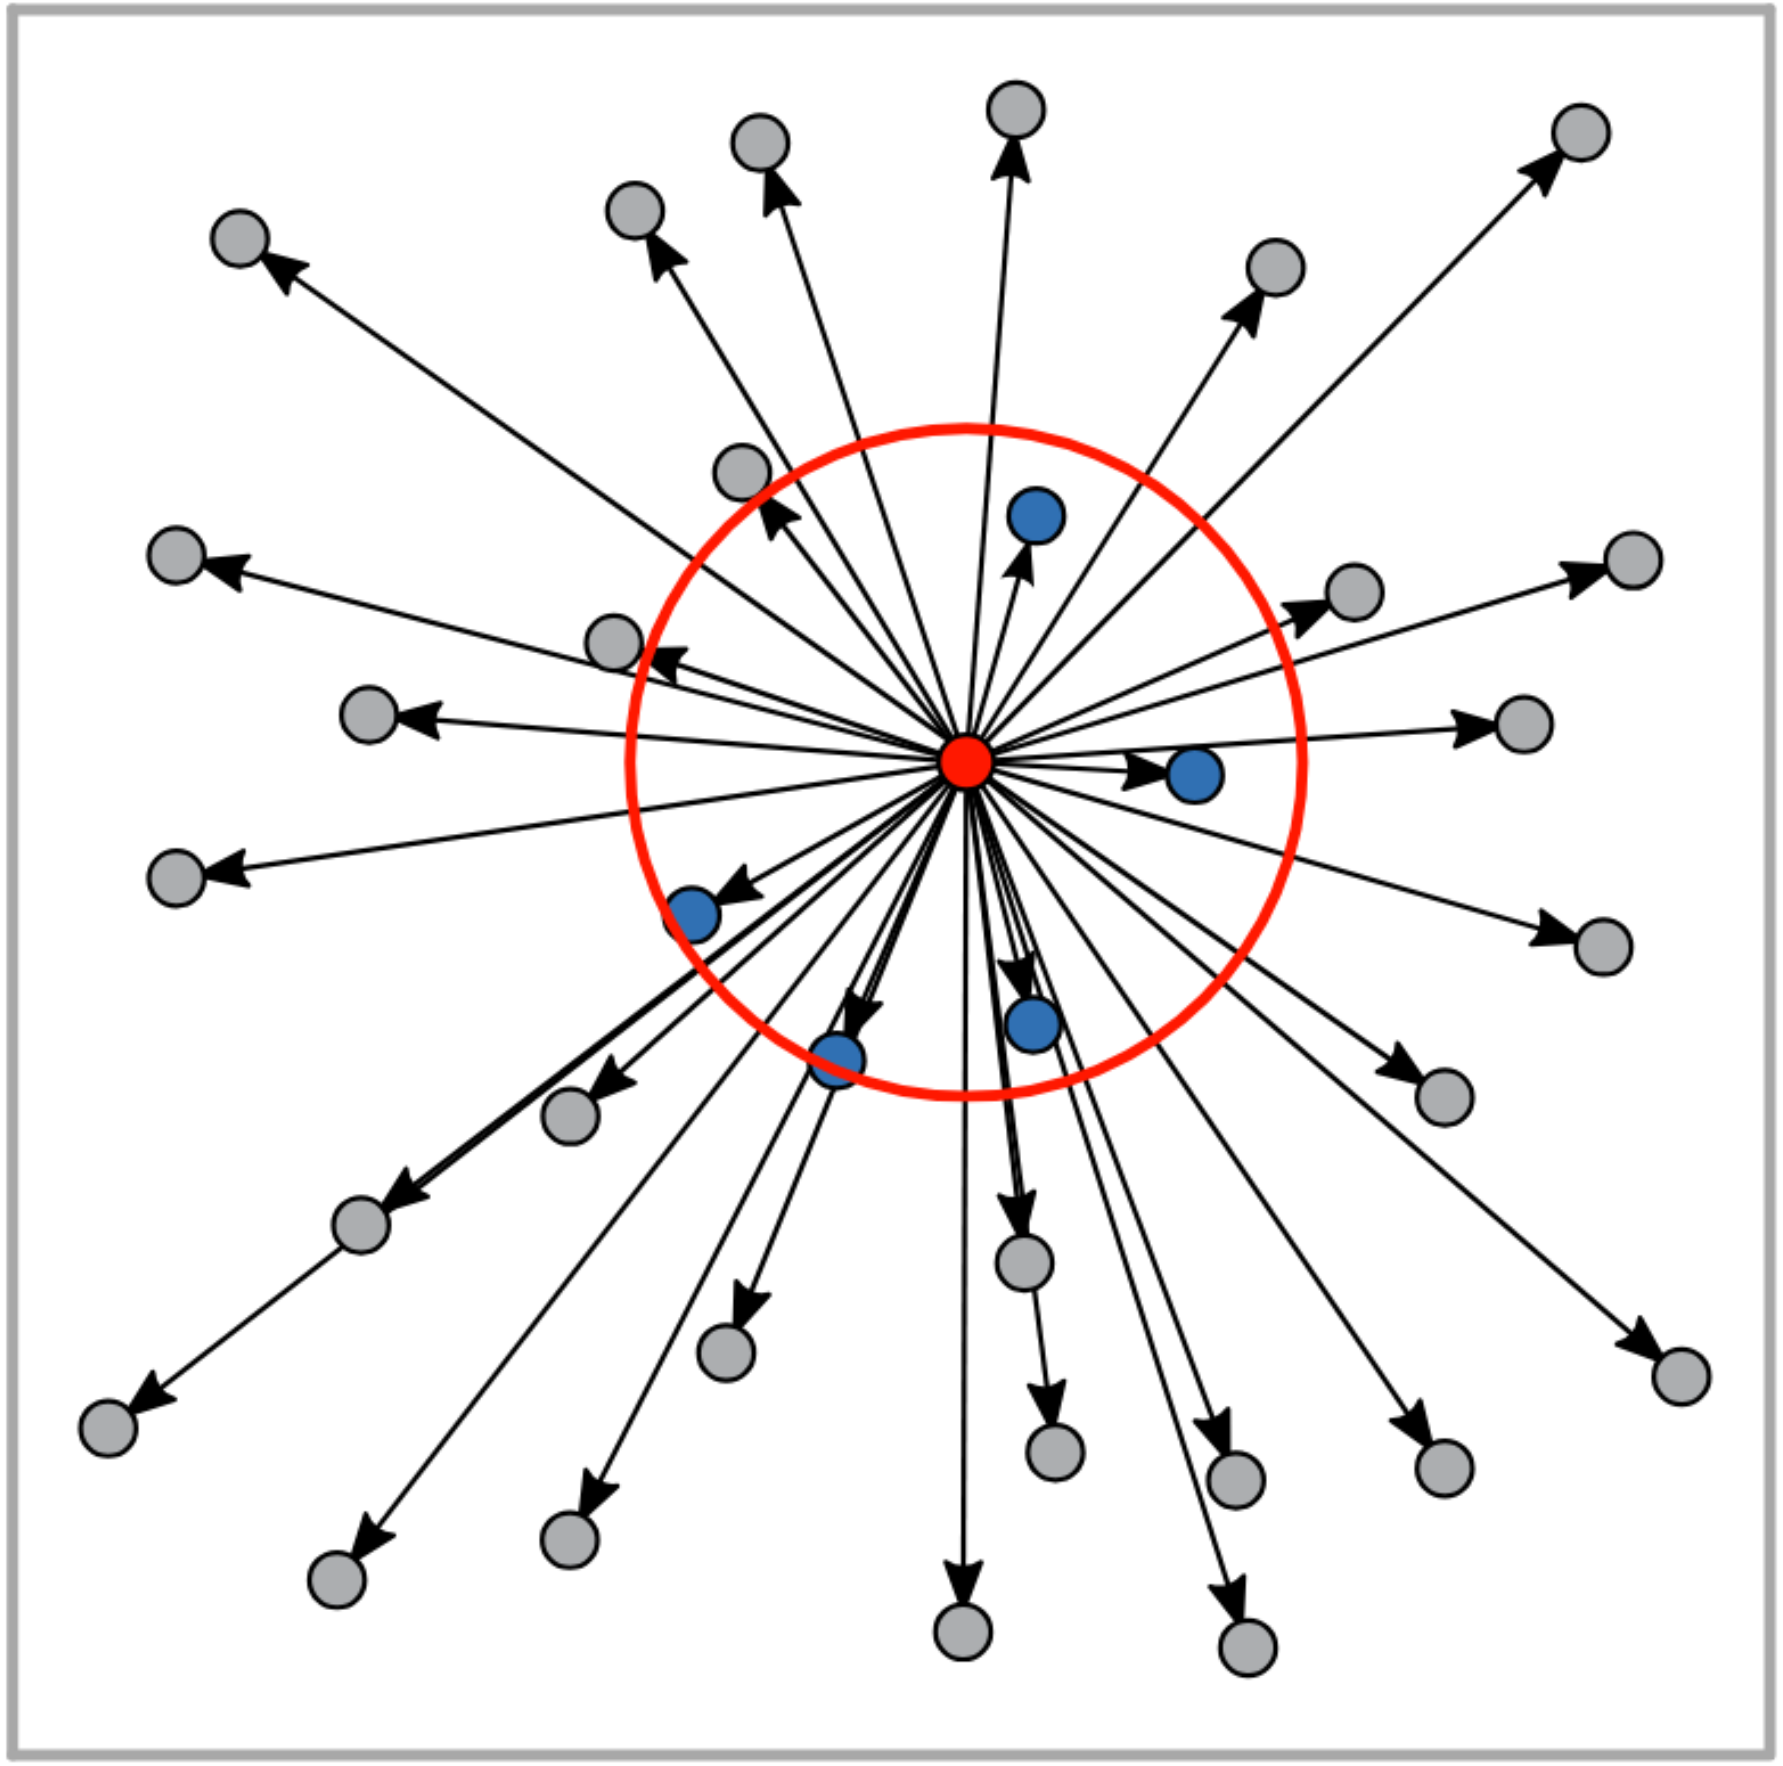
\includegraphics[width=\linewidth]{imgs/directsum.png}
        \caption{\scriptsize Direct Sum}
        \label{fig:directsum}
    \end{subfigure}
    \hfill
    % Second Figure
    \begin{subfigure}{0.22\textwidth}
        \centering
        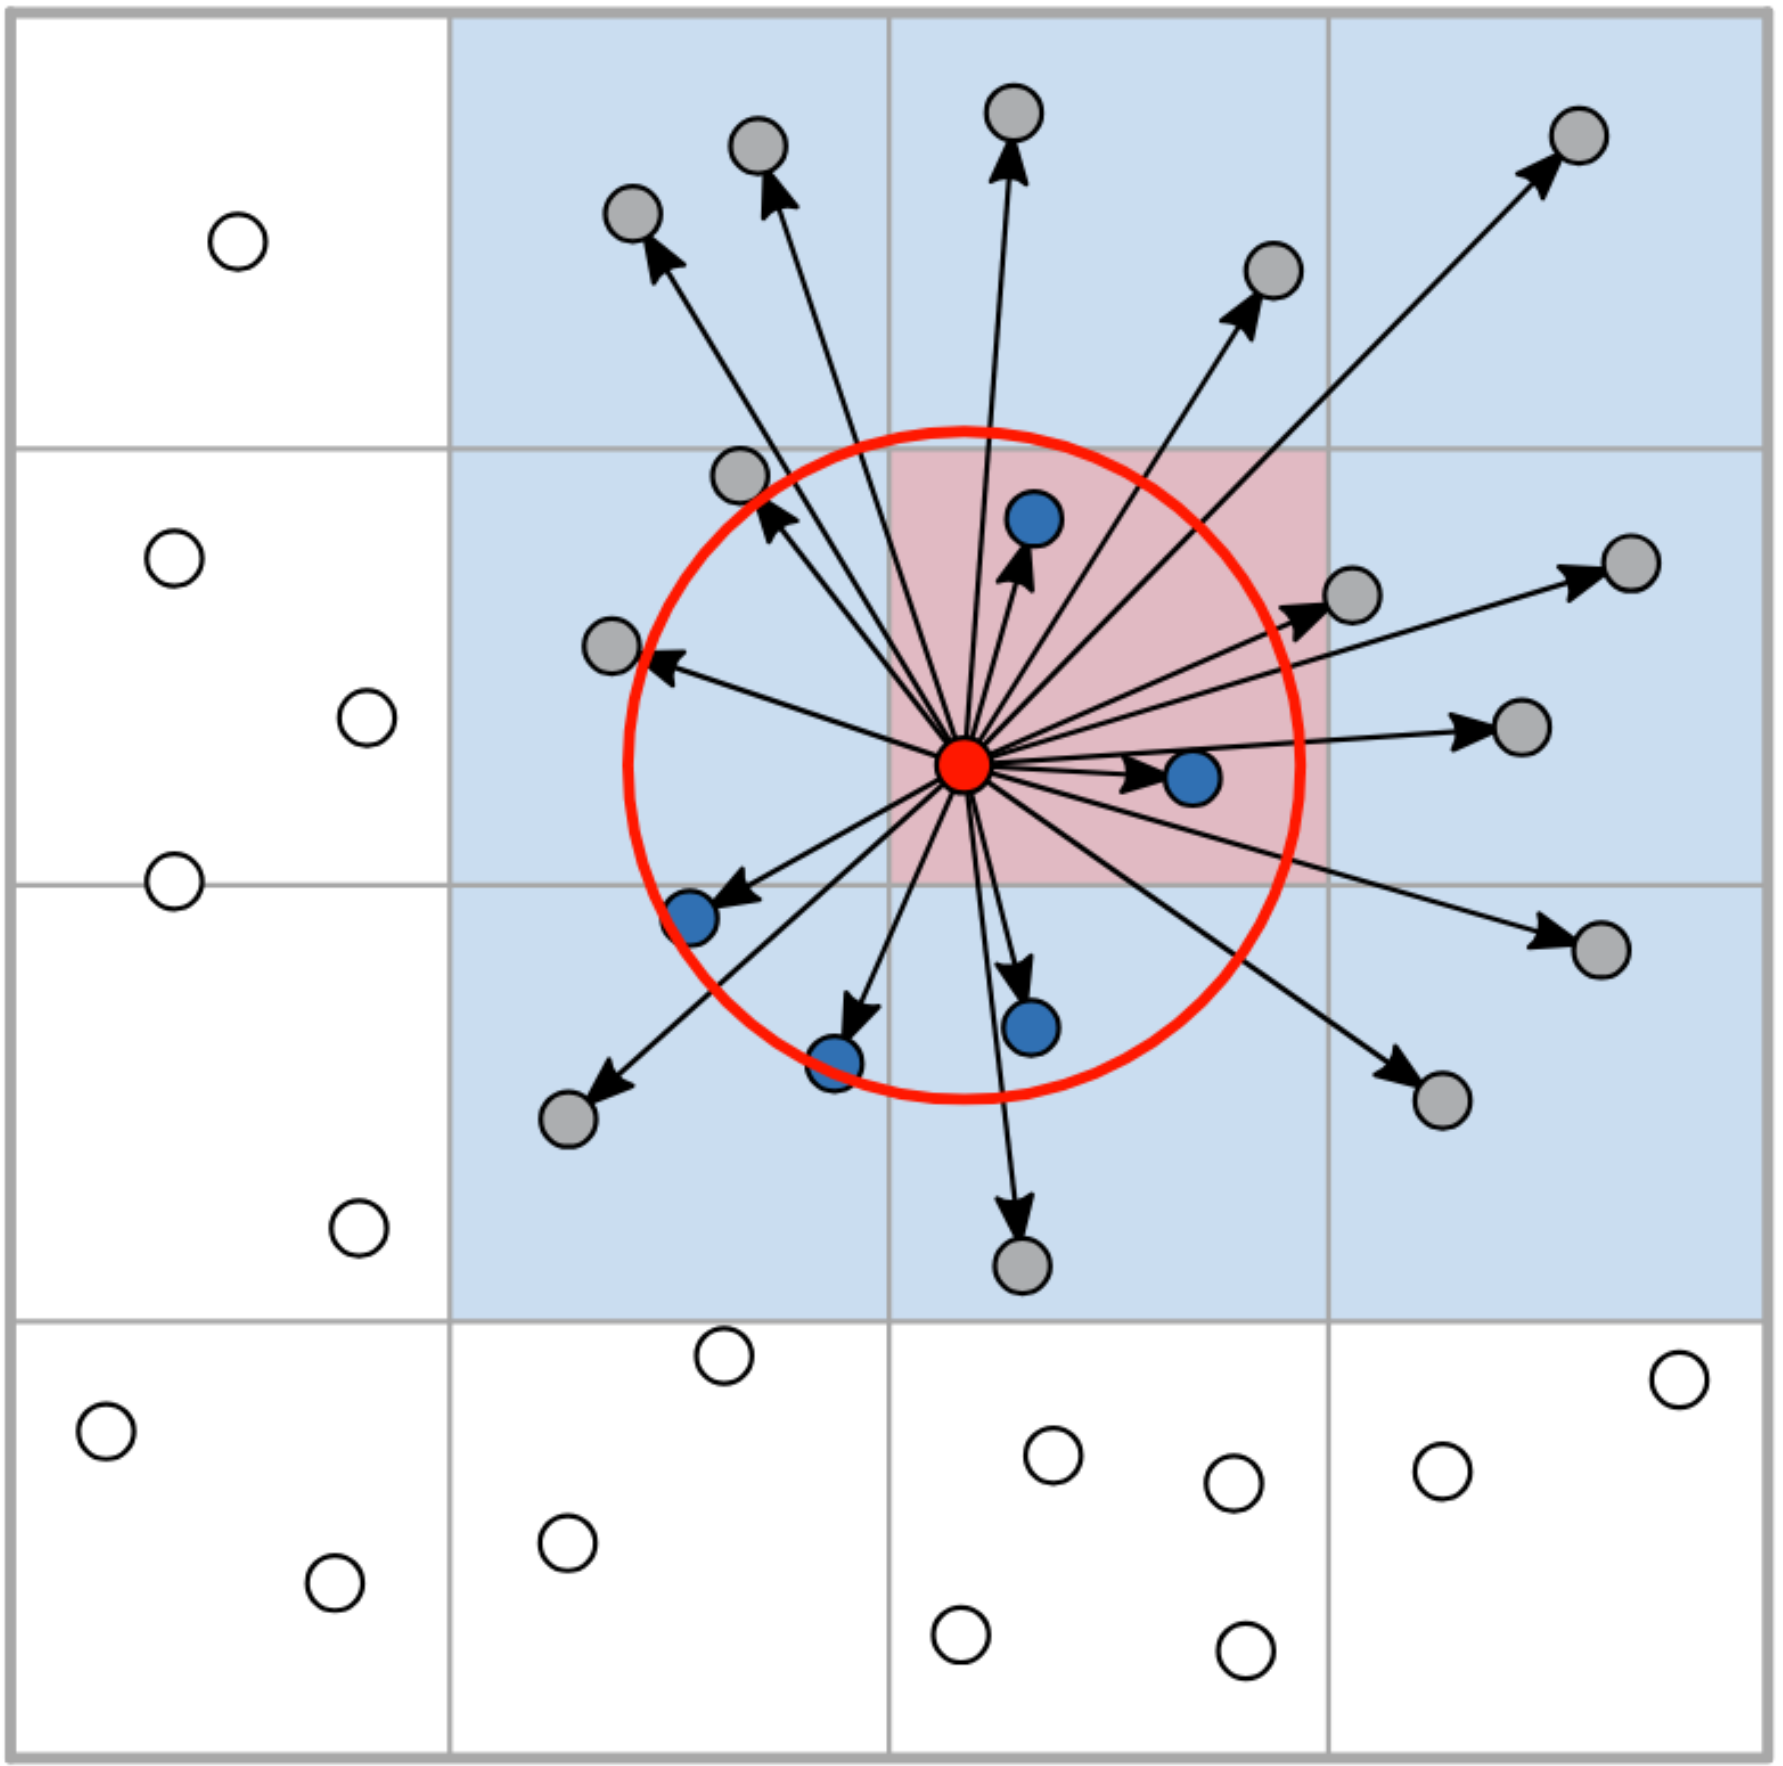
\includegraphics[width=\linewidth]{imgs/linkedcells.png}
        \caption{\scriptsize Linked Cells}
        \label{fig:linkedcells}
    \end{subfigure}
    \hfill
    % Third Figure
    \begin{subfigure}{0.22\textwidth}
        \centering
        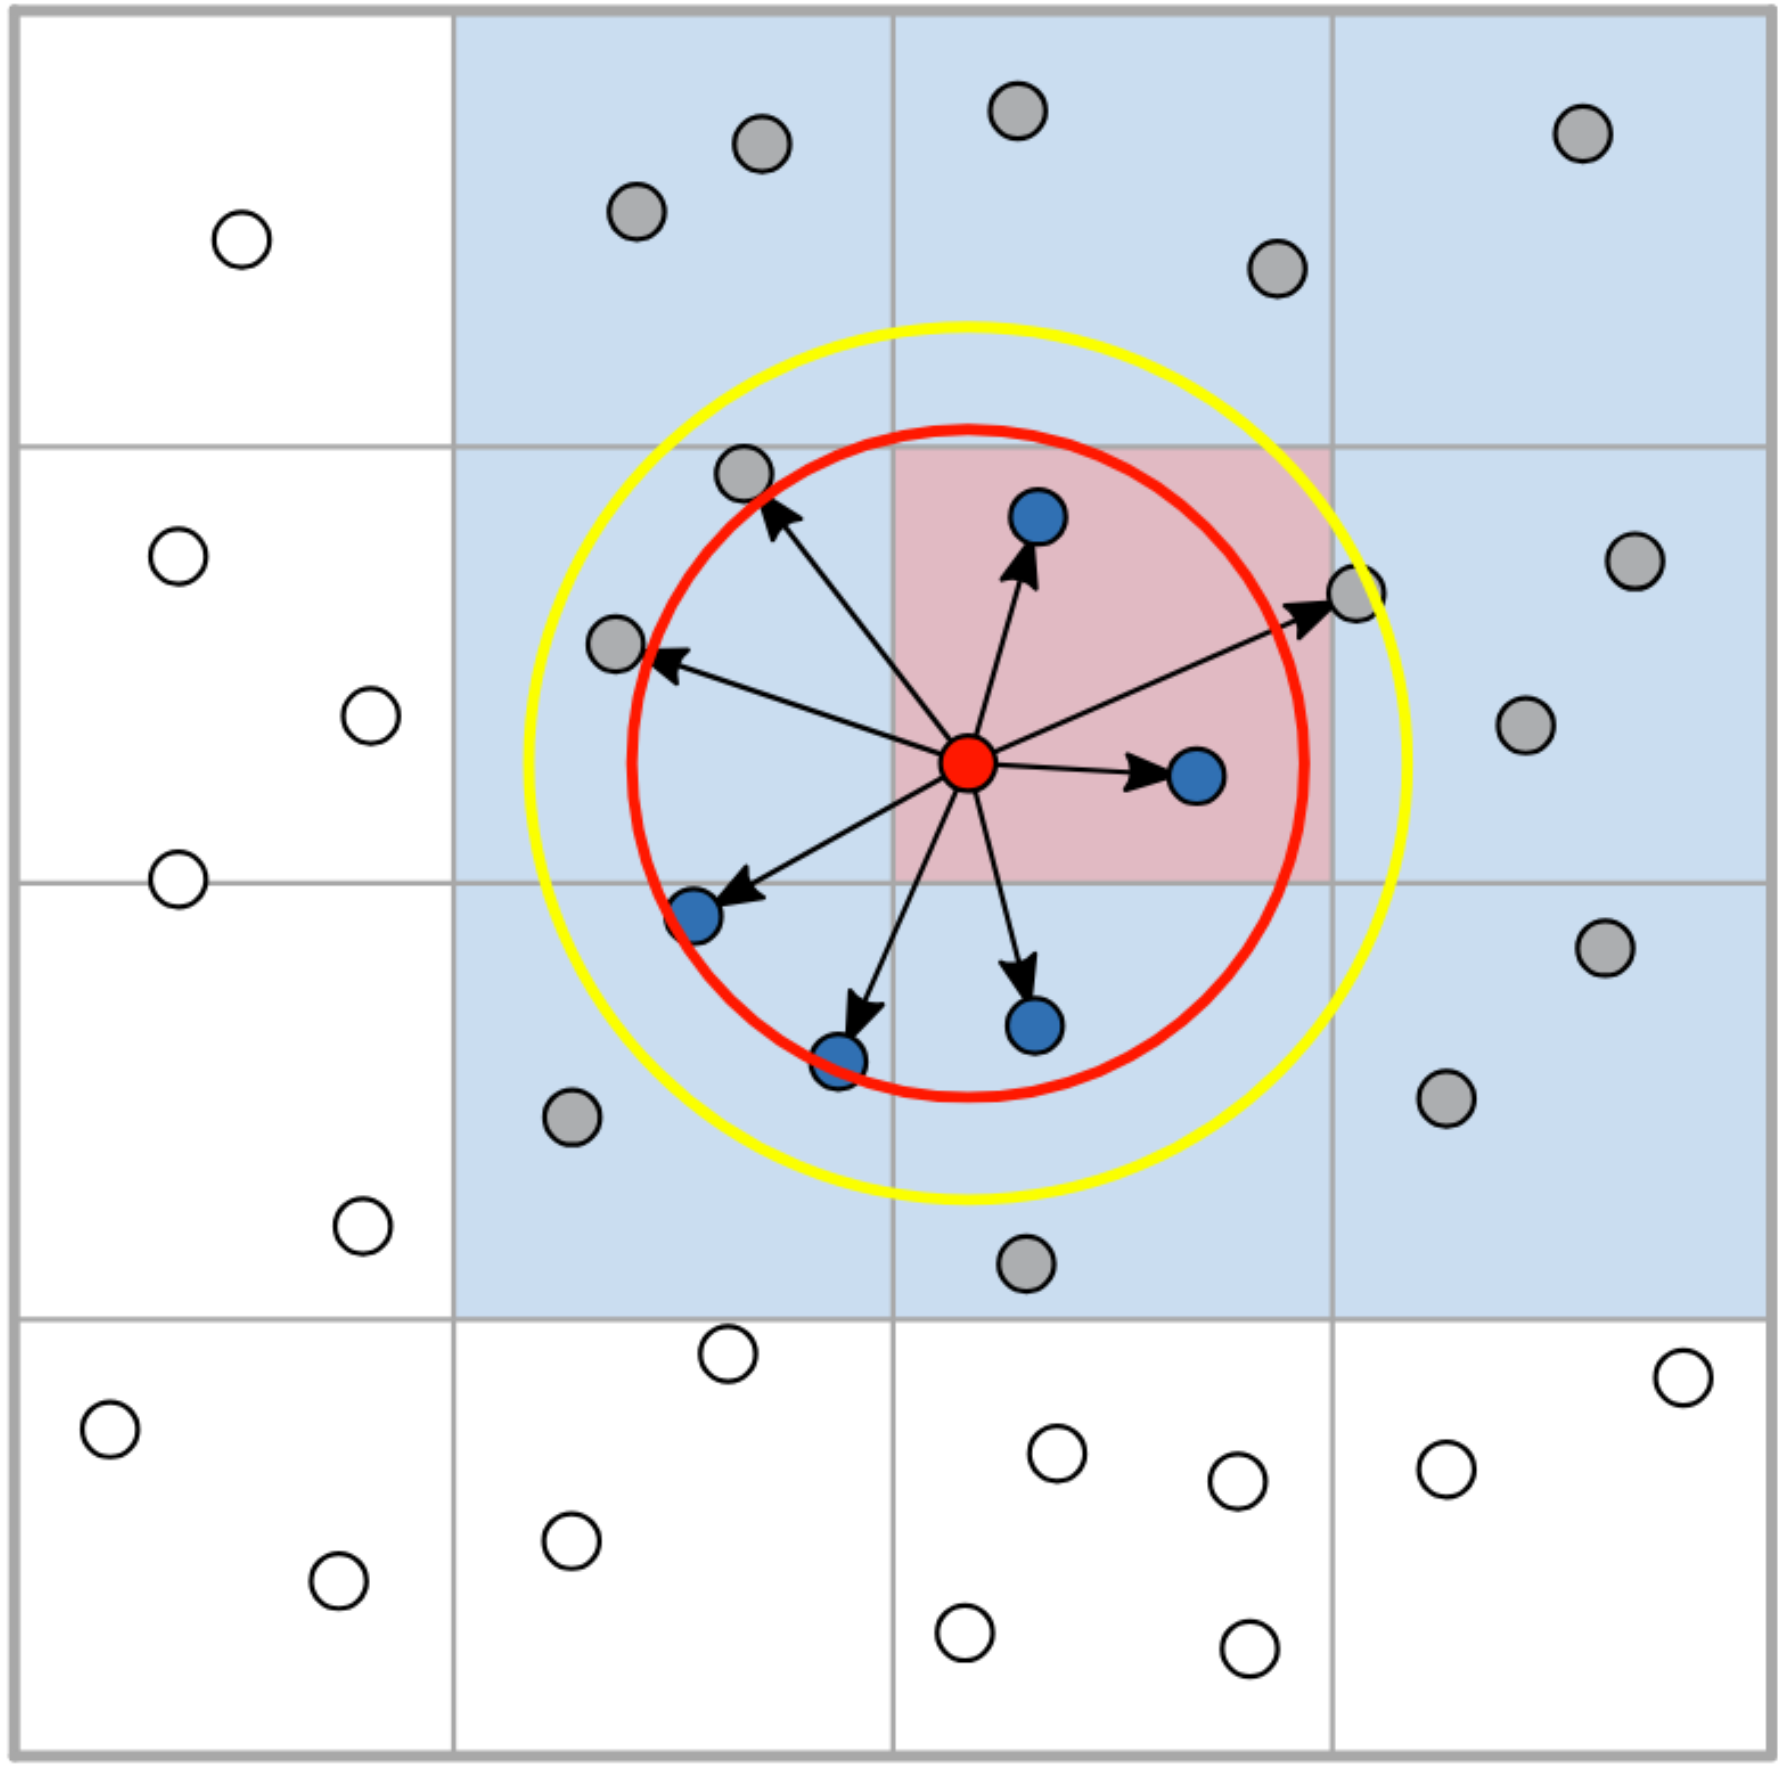
\includegraphics[width=\linewidth]{imgs/verletlists.png}
        \caption{\scriptsize Verlet Lists}
        \label{fig:verletlists}
    \end{subfigure}
    \hfill
    % Fourth Figure
    \begin{subfigure}{0.22\textwidth}
        \centering
        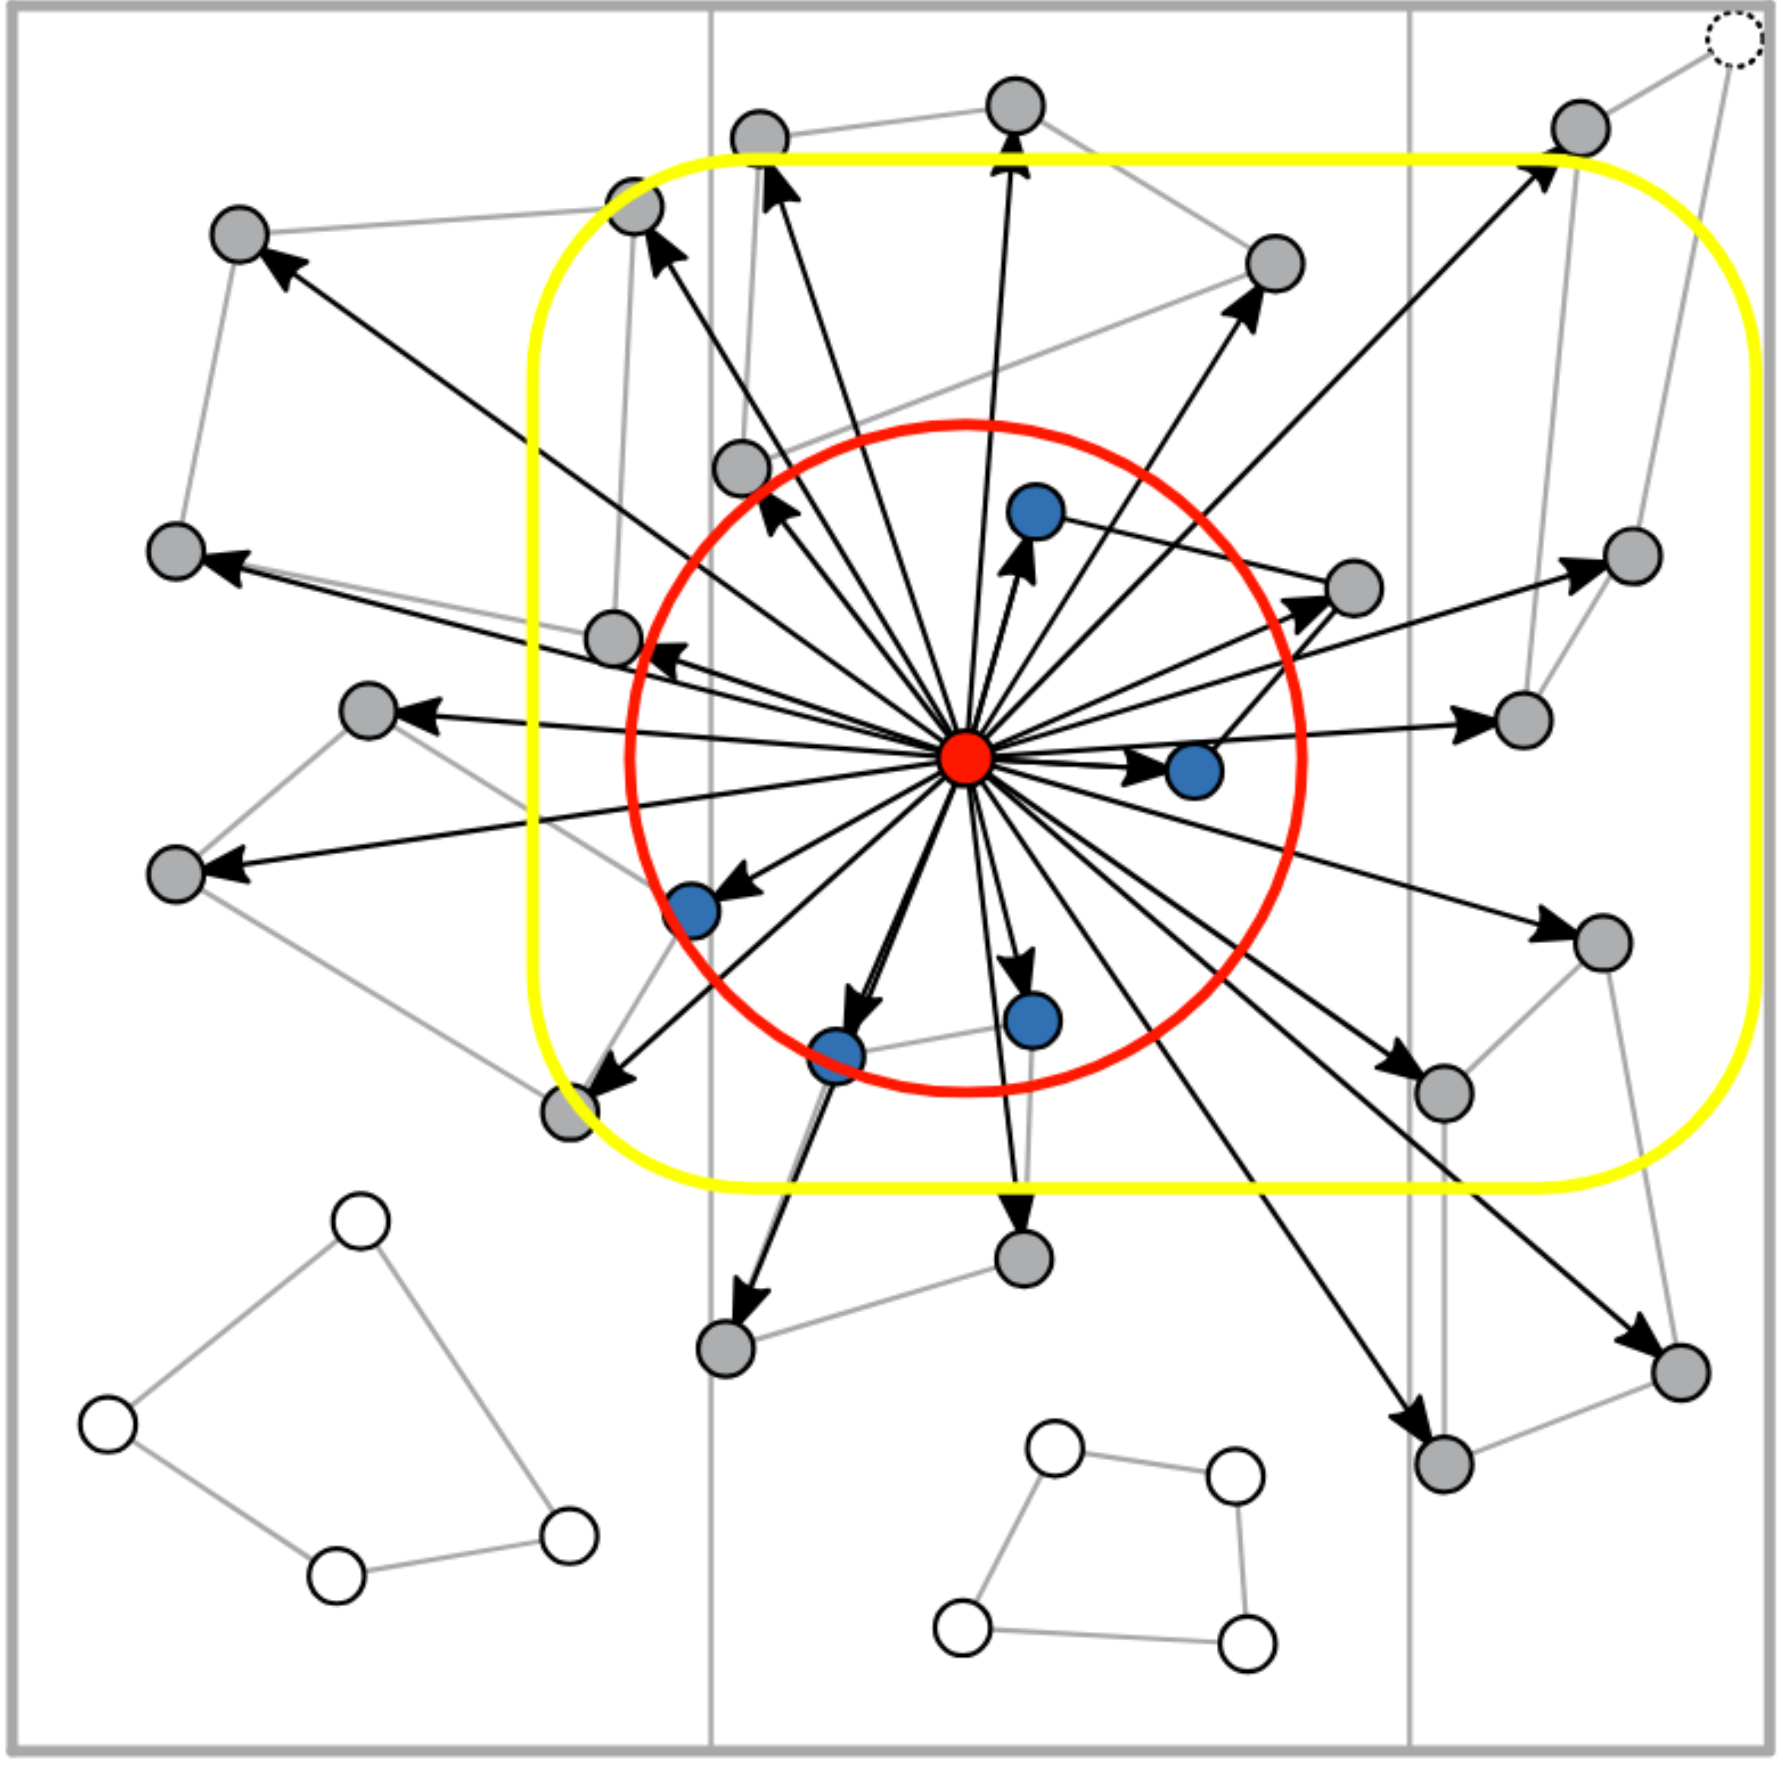
\includegraphics[width=\linewidth]{imgs/verletclusters.png}
        \caption{\scriptsize Verlet Cluster Lists}
        \label{fig:verletclusters}
    \end{subfigure}
    \caption{Neighbor Identification Algorithms in AutoPas \parencite{gratl2022n}}
\end{figure}



\subsection{Traversals}

Traversals determine the order in which particle interactions are computed. AutoPas supports a variety of traversal strategies, each specific to the container being used. These strategies are designed to optimize performance by parallelizing the traversal process, while avoiding race conditions and minimizing the need for schedulers or locking mechanisms \parencite{gratl2019autopas}.

Traversal strategies in AutoPas utilize different cell strategies as their base step. The goal of these base steps is to divide and color the cells of the domain, such that particles in cells of the same color can be processed independently by separate threads. Currently, AutoPas implements three types of base steps: c01, c18, and c08; however, for this thesis, only c01 and c08 are relevant.

\subsection{Base Steps in AutoPas}

\subsubsection{c01 Base Step} The c01 base step uses only a single color, as illustrated in Figure \ref{fig:c01}, and calculates interactions for all neighboring cells without utilizing the Newton3 optimization. In this approach, each cell is assigned to a thread, which calculates the interactions with particles in the neighboring cells. This strategy is highly parallelizable.

% \subsubsection{c18 Base Step} The c18 base step assigns one of 18 colors to each cell, ensuring that no two neighboring cells share the same color. By utilizing the Newton3 optimization, the number of interactions to be calculated is reduced by half. Instead of processing all neighbors, it focuses only on neighbors with a higher index (see Figure~\ref{fig:c18}). This reduces the overall number of computations, however increases the area where race conditions need to be managed, limiting parallel execution.

\subsubsection{c08 Base Step} As the name suggests, the c08 base step uses 8 colors. It is similar to c18 but reduces the locked area further by limiting diagonal interactions and focusing on only four cells (see Figure~\ref{fig:c08}). This adjustment allows for better parallel processing and improved cache utilization.


\subsection{Traversal Strategies}
This thesis focuses on the traversals \texttt{lc\_c08}, \texttt{vlc\_c08}, and \texttt{vcl\_c06}, as they were extensively used in the experiments conducted. A detailed explanation of these strategies is provided below. For information on all traversal strategies, refer to \parencite{gratl2022n}.

\subsubsection{\texttt{lc\_c08}}
This traversal utilizes \texttt{c08} as its base step, and it is designed for the Linked Cells container. It divides a 2D domain into four colors and a 3D domain into eight colors. The dependency of the number of colors \(C\) on the number of dimensions \(D\) follows \(C = 2^D\) \parencite{gratl2022n}.

\subsubsection{\texttt{vlc\_c08}}
This traversal applies the \texttt{c08} base step to each individual cell. To ensure thread safety, a domain coloring consisting of eight colors is used. For each cell, all neighbor lists are processed. Depending on whether the lists were built with Newton3, the base step used is either c01 or c08. \parencite{AutoPasDocs}

\subsubsection{\texttt{vcl\_c06}}
This traversal is used for Verlet Cluster Lists, and it employs a 2D coloring scheme with a stride of \(x = 3\) and \(y = 2\), resulting in six colors (\(3 \times 2 = 6\)). Interactions within clusters are always computed using Newton3, regardless of whether Newton3 is enabled or disabled for the overall traversal. \parencite{AutoPasDocs}

\begin{figure}[htbp]
    \centering
    \begin{subfigure}[b]{0.25\textwidth}
        \centering
        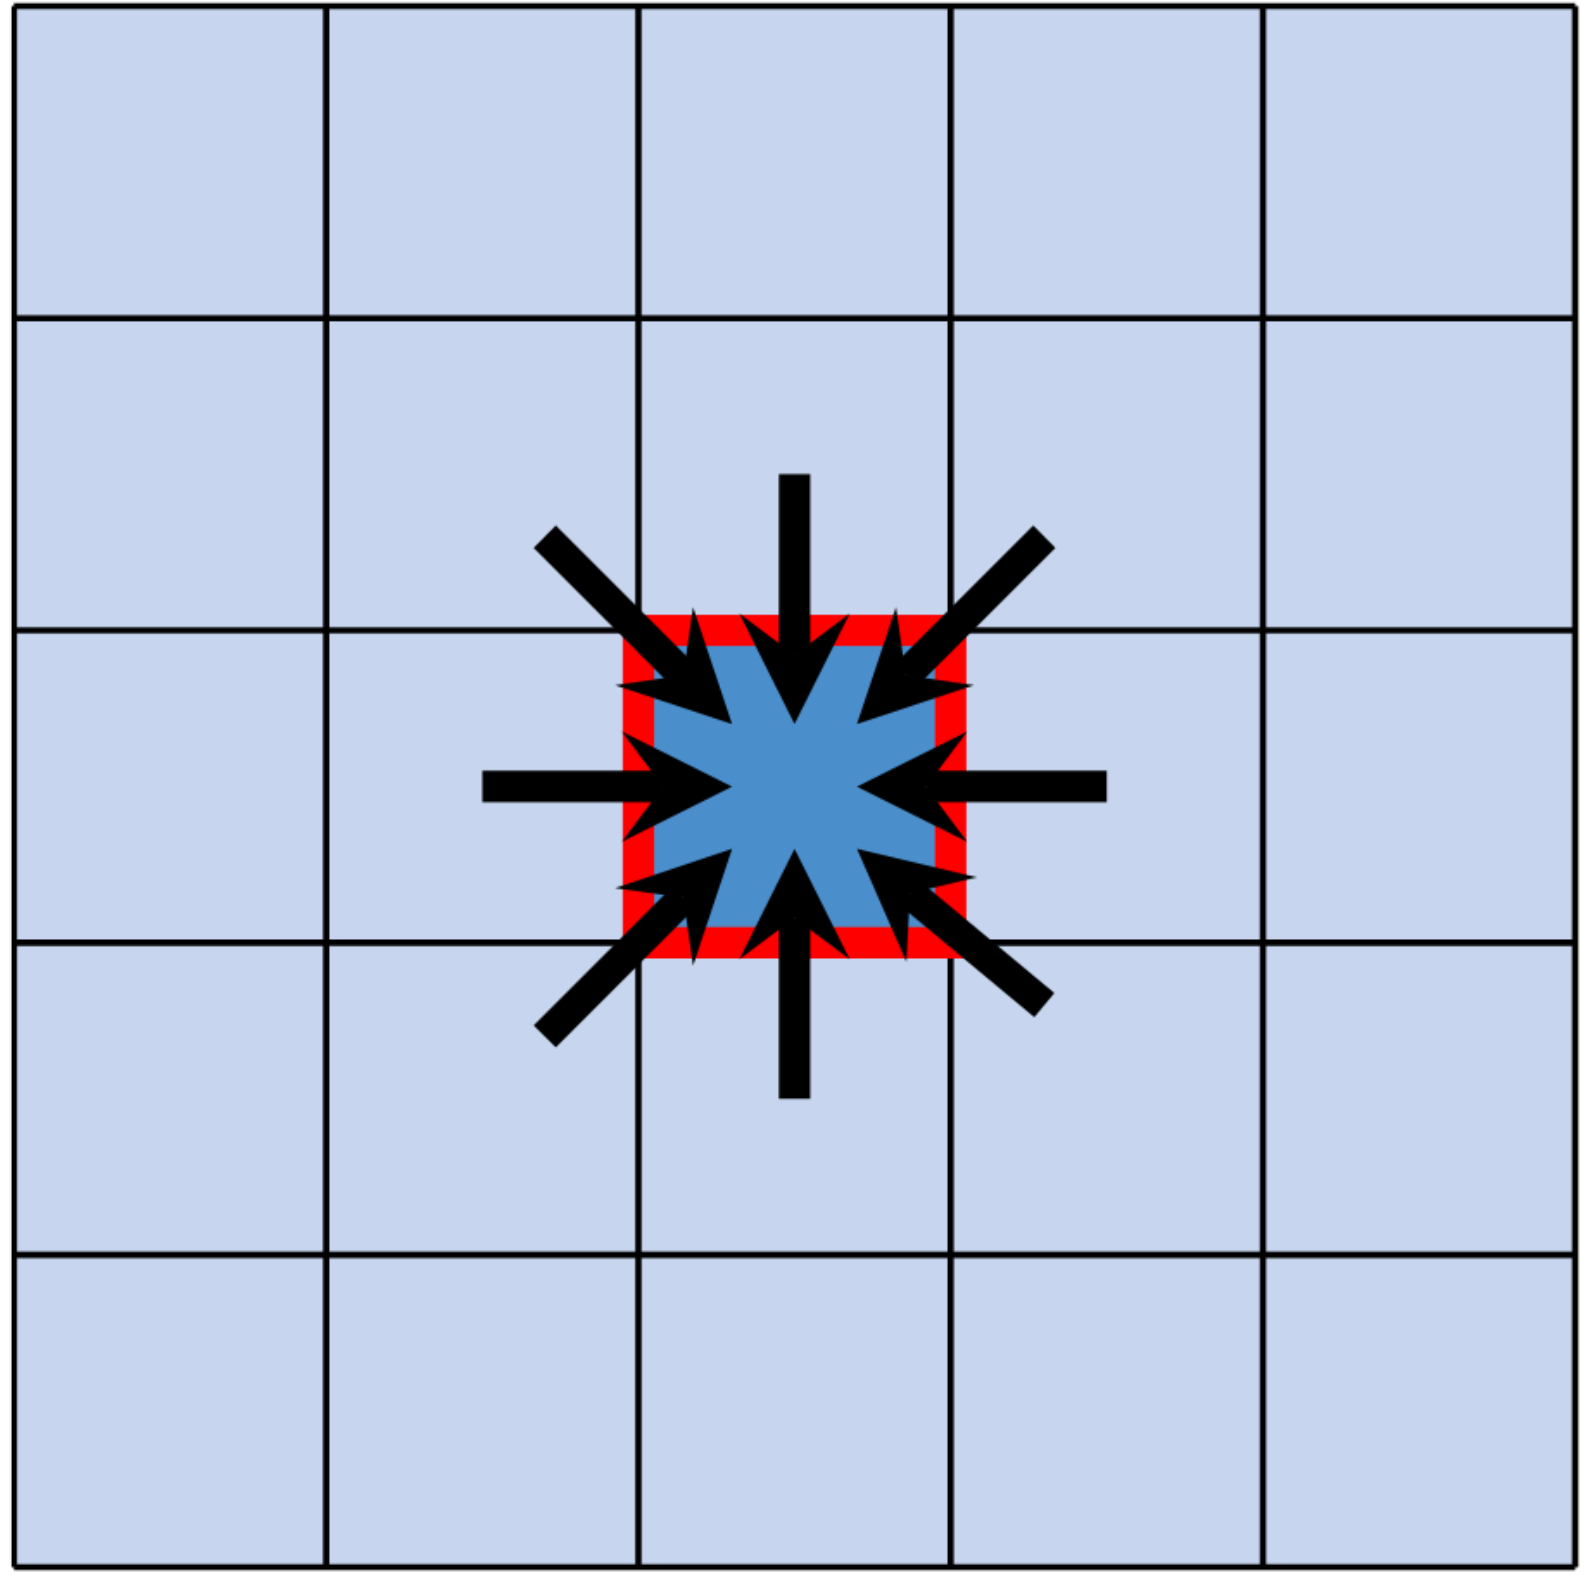
\includegraphics[width=\linewidth]{imgs/c01.png}
        \caption{\scriptsize c01 base step}
        \label{fig:c01}
    \end{subfigure}
    % \begin{subfigure}[b]{0.3\textwidth}
    %     \centering
    %     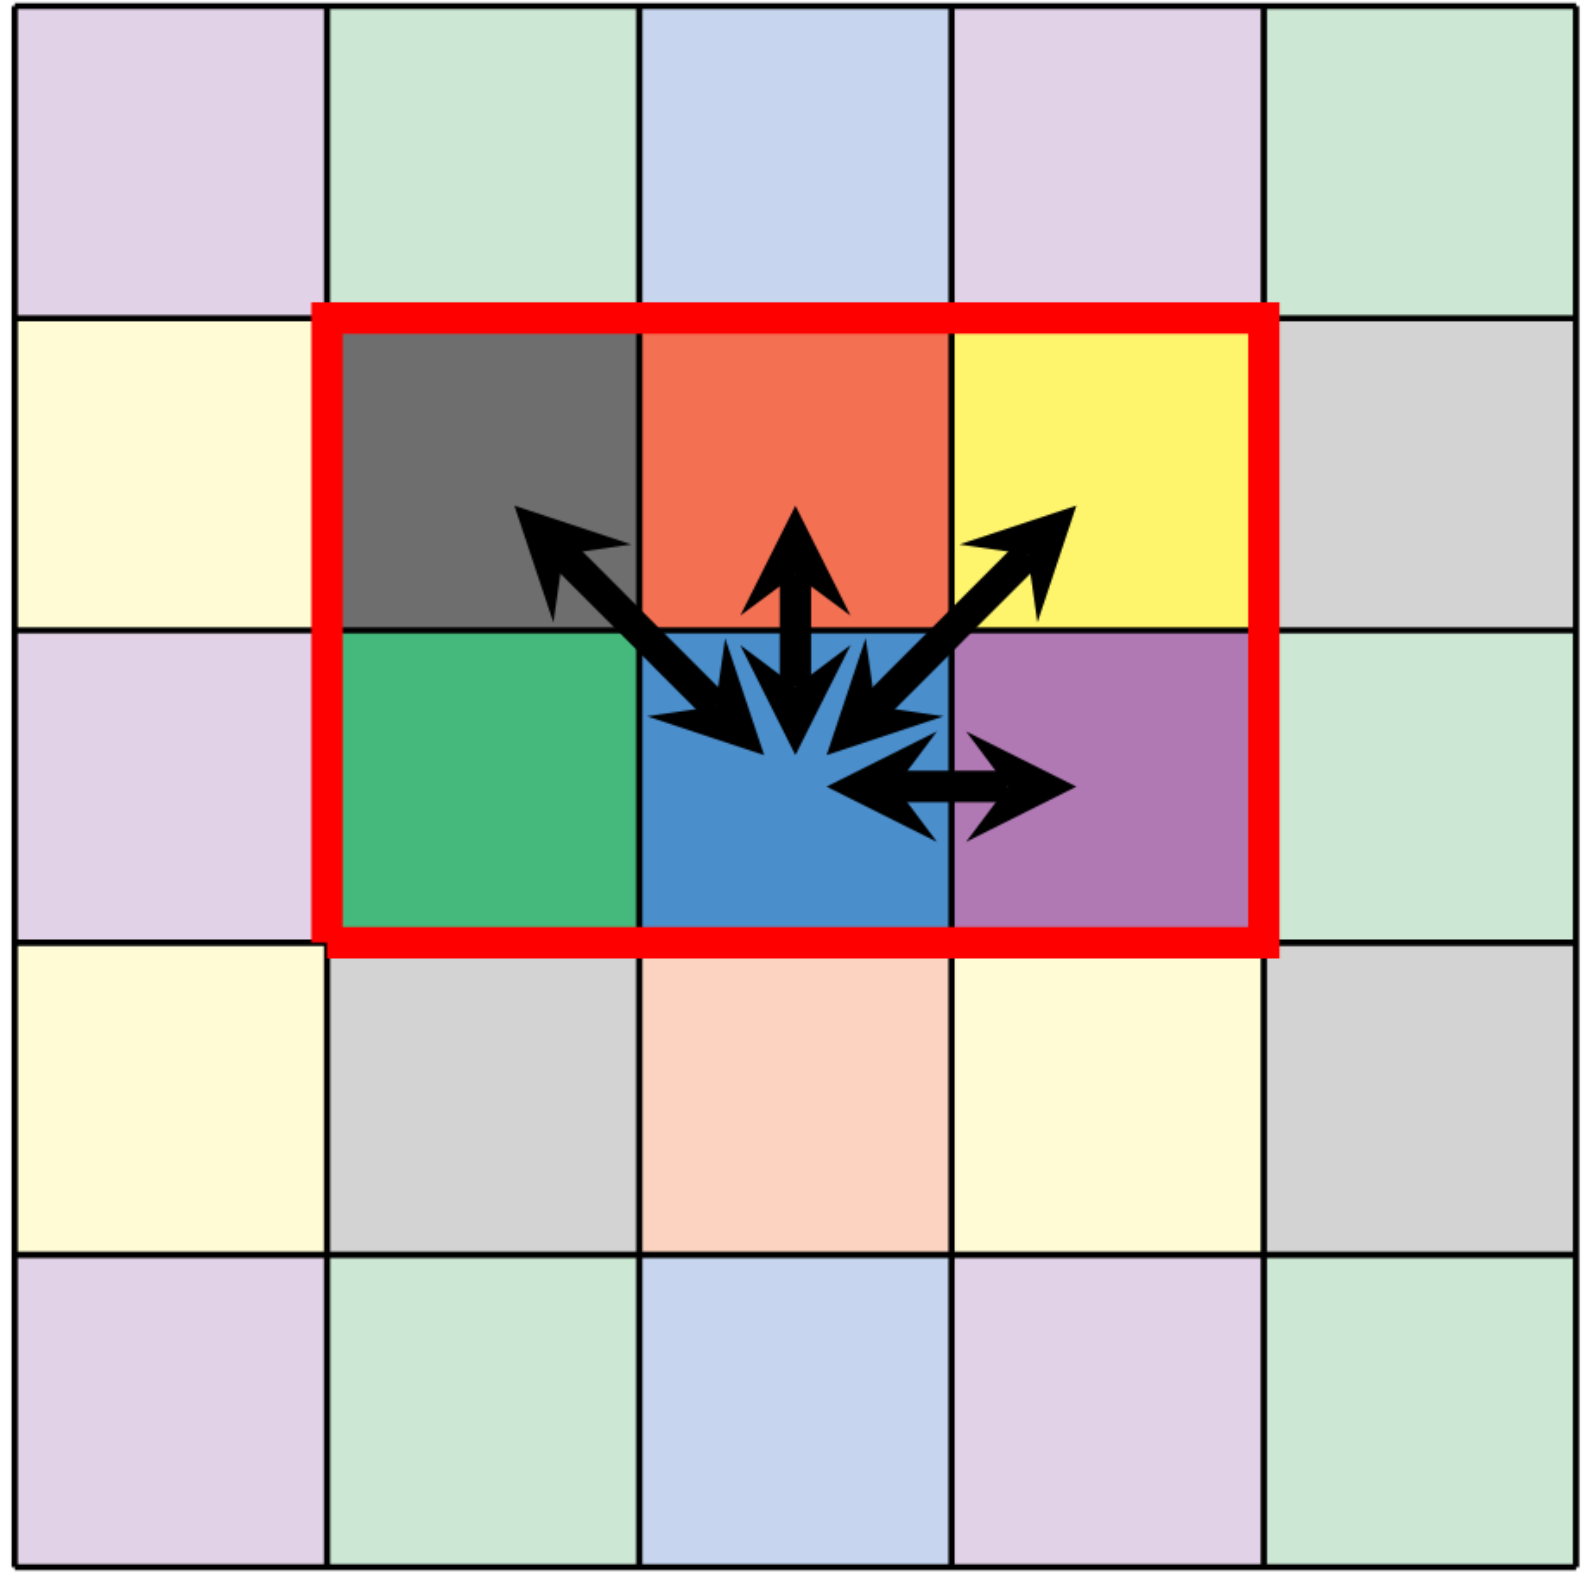
\includegraphics[width=\linewidth]{imgs/c18.png}
    %     \caption{\scriptsize c18 base step}
    %     \label{fig:c18}
    % \end{subfigure}
    \hspace{1em}
    \begin{subfigure}[b]{0.25\textwidth}
        \centering
        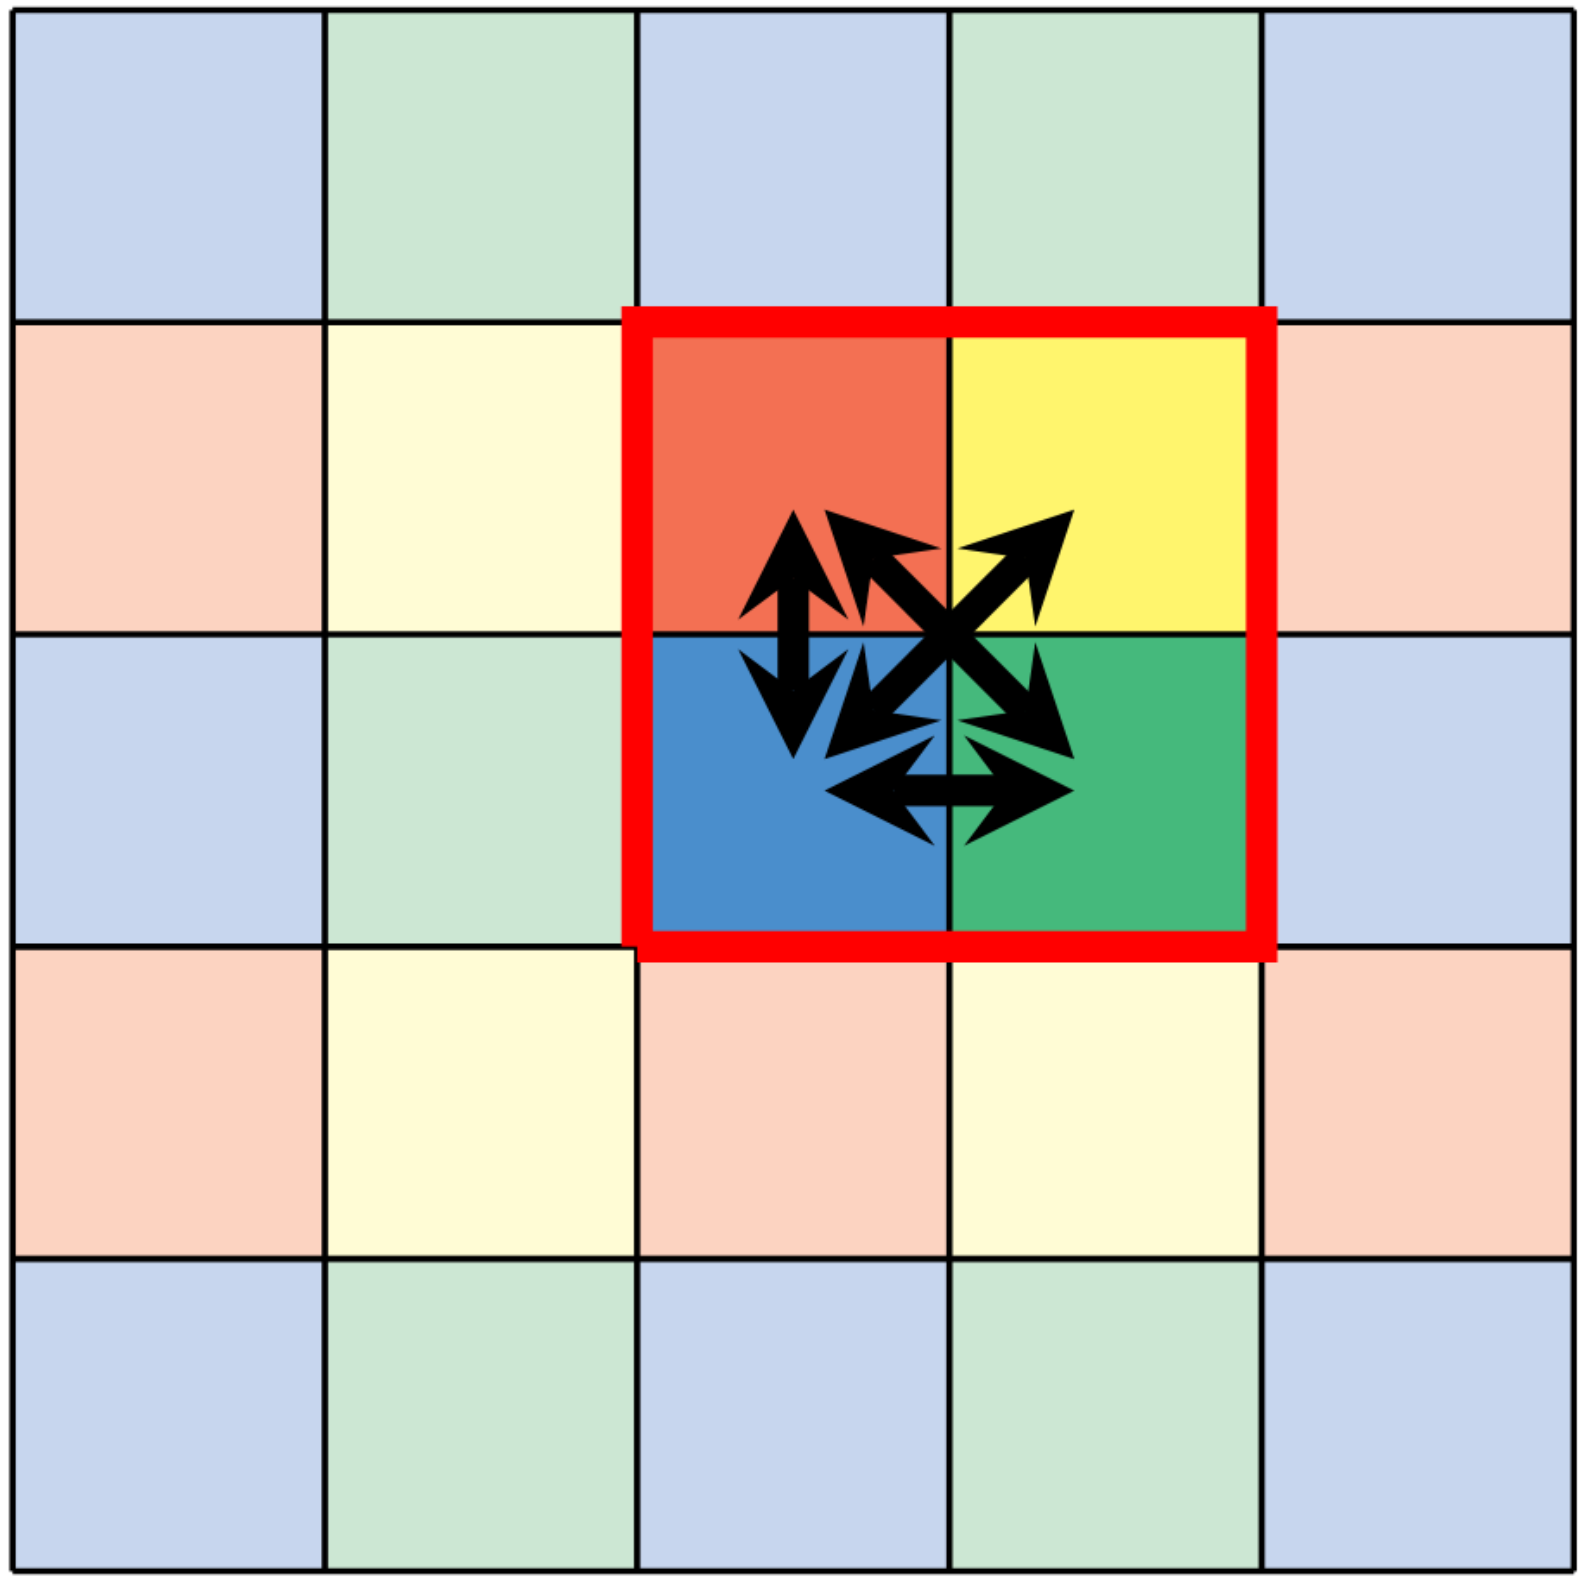
\includegraphics[width=\linewidth]{imgs/c08.png}
        \caption{\scriptsize c08 base step}
        \label{fig:c08}
    \end{subfigure}
    \caption{Base Step Approaches \parencite{newcome2023towards}}
\end{figure}



\subsection{Auto-Tuning}

One of the key features of AutoPas is its auto-tuning capability. Choosing the optimal combination of container and traversal for a simulation can be challenging, especially since different parts of the simulation may benefit from different configurations. AutoPas automates this process, relieving the user of the need to determine the best setup manually.

At the beginning of a simulation, AutoPas tests various configurations over a few iterations, measuring their performance. To reduce overhead, configurations using the same container are tested consecutively. This approach assumes that the state of the simulation remains relatively stable over consecutive time steps, making the performance results comparable. Importantly, the results of these initial tests are not discarded but are used in the following iterations \parencite{gratl2019autopas}.

After evaluating multiple configurations, AutoPas selects the best-performing setup and uses it for a user-defined number of iterations. Following this period, the system enters a re-tuning phase, where a new configuration may be selected based on how the simulation has evolved.








\subsection{Particle Types}

In AutoPas, there are three types of particles: Owned, Halo, and Dummy particles.  
\begin{itemize}
    \item Owned particles are the primary particles managed by the current AutoPas instance. These represent the actual simulation particles within a subdomain.  
    \item Halo particles are not owned by the current AutoPas object but exist at the borders of subdomains. Since they interact with particles in neighboring domains, they must be duplicated and made available in neighboring subdomains to ensure the correct computation of forces. During force calculations, halo particles serve as interaction partners like any other particle, but their forces are only computed in the domain that owns them.  
    \item Dummy particles represent deleted particles. They do not participate in force calculations.

\end{itemize}


\subsection{Interaction Computation in AutoPas} \label{sec:interaction_comp}

Two important buffers are used in AutoPas: the particle buffer and the halo particle buffer. The particle buffer stores particles that should not yet be added to the container. The halo particle buffer holds halo particles, making sure that particles at the boundaries of subdomains are available for correct force calculations.


In AutoPas, interactions are computed in two stages so that all particles are correctly accounted for during the simulation.

\begin{enumerate}
    \item \textbf{Container Interactions}: The main function \texttt{computeInteractions(\&traversal)} calculates interactions for particles within the container. This involves iterating over particle pairs, triplets, or higher multiples, ensuring efficient resolution of regular particle interactions.

    \item \textbf{Buffer Interactions}: Interactions for particles in the buffers are computed separately using the \texttt{computeRemainderInteractions(functor, newton3)} function. This step ensures that particles in the buffer interact correctly with container particles and among themselves. The following types of interactions are handled:
    \begin{itemize}
        \item \textbf{Particle Buffer \(\leftrightarrow\) Container}: Interactions between buffer particles and container particles.
        \item \textbf{Halo Particle Buffer \(\rightarrow\) Container}: Interactions from halo particle buffers to container particles.
        \item \textbf{Particle Buffer \(\leftrightarrow\) Particle Buffer}: Interactions among buffer particles.
        \item \textbf{Halo Particle Buffer \(\rightarrow\) Particle Buffer}: Interactions from halo particle buffers to buffer particles.
    \end{itemize}
\end{enumerate}

% This two-stage computation guarantees accurate interaction handling for all particles, including those in the buffers. Explicit handling of buffer particles allows the simulation to avoid unnecessary neighbor list rebuilds, maintaining computational efficiency.


